\documentclass[]{article}

\usepackage{amsmath}
\usepackage{amsfonts}
\usepackage{tikz}
\usepackage{float}
\usepackage{parskip}
%opening
\title{}
\author{}

\newcommand{\thetahat}{\hat{\theta}^{(t)}}

\usetikzlibrary{fit,positioning,arrows,automata,calc}
\tikzset{
  main/.style={circle, minimum size = 5mm, thick, draw =black!80, node distance = 10mm},
  connect/.style={-latex, thick},
  box/.style={rectangle, draw=black!100}
}

\begin{document}

\maketitle


Let's restate the general EM algorithm. First, we had the E-step:
$$Q(\theta, \thetahat) = \mathbb{E}_{z \mid x; \thetahat}
\big[\ln L(\theta; x,z)\big]$$
Where $z$ are latent variables, and $x$ are observed variables. Then, the M-step is
$$\theta^{(t+1)} = \arg\max_{\theta} Q(\theta, \thetahat)$$

We want to apply this algorithm to our Gaussian Mixture Model, where
$$p(x_i \mid z_i) = \prod_{j=1}^{J} \mathcal{N}(x_i \mid \mu_j, \Sigma_j)^{z_{ij}}$$
where $J$ is the number of labels (or Gaussians) we have. We have
$$p(z_{ij} = 1) = \tau_{j}$$
where $\tau_j$ is a probability vector. This gives us 
$$p(z_{i}) = \prod_{j=1}^J = \tau_j^{z_{ij}}$$


We can draw the variable diagram as
\begin{figure}[H]
\centering
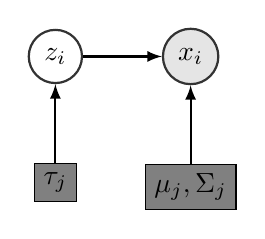
\begin{tikzpicture}
  \node[main] (Latent) {$z_i$};
  \node[main,fill=black!10] (Observed) [right=of Latent] {$x_i$};
  \path (Latent) edge [connect] (Observed);
    \node[box,fill=black!50] (Lvar) [below=of Latent] {$\tau_{j}$};
    \node[box,fill=black!50] (Ovar) [below=of Observed] {$\mu_j, \Sigma_j$};
    
    \path (Ovar) edge [connect] (Observed);
    
    \path (Lvar) edge [connect] (Latent);
\end{tikzpicture}
\caption{$\theta_j = (\tau_j, \mu_j, \Sigma_j)$}
\end{figure}

Next, we can compute the likelihood as

\begin{align*}
L(\theta; x,z) &= \prod_{i=1}^N p(x_i \mid z_i; \theta)p(z_i;\theta)\\
&= \prod_{i=1}^N\prod_{j=1}^J \tau_j^{z_{ij}} \mathcal{N}(x_i; \mu_j, \Sigma_j)^{z_{ij}}
\end{align*}

Then, for our E-step we need to compute the log likelihood,

$$\ln(L(\theta; x,z)) = \sum_{i=1}^N\sum_{j=1}^J z_{ij}\Big(\ln\tau_j + \ln \mathcal{N}(x_i; \mu_j, \Sigma_j)\Big)$$
And we need to compute
\begin{align*}
p(z_{ij} = 1 \mid x_i; \thetahat) &= \frac{p(x_i \mid z_{ij})P(z_{ij} = 1)}{p(x_i)}\\
&= \frac{\hat{\tau}_j \mathcal{N}(x_i; \hat{\mu_j}, \hat{\Sigma_j})}{\sum_{j=1}^{J} \hat{\tau}_j \mathcal{N}(x_i; \hat{\mu_j}, \hat{\Sigma_j})}\\
&\hat{=}~ p_{ij}
\end{align*}

Then
\begin{align*}
Q(\theta, \thetahat) &= \mathbb{E}_{z \mid x; \thetahat}
\Bigg[ \sum_{i=1}^N\sum_{j=1}^J z_{ij}\Big(\ln\tau_j + \ln \mathcal{N}(x_i; \mu_j, \Sigma_j)\Big)\Bigg]\\
&=  \sum_{i=1}^N\sum_{j=1}^J \Big(\ln\tau_j + \ln \mathcal{N}(x_i; \mu_j, \Sigma_j)\Big)\mathbb{E}_{z \mid x; \thetahat}[z_{ij}]
\end{align*}
and $\mathbb{E}_{z \mid x; \thetahat}[z_{ij}] = p_{ij}$.

Now for the M-step, we want to calculate $\frac{d}{\mu_j}$, $\frac{d}{\Sigma_j}$, and $\frac{d}{\tau_j}$.

\begin{align*}
0 &= \frac{d}{\mu_j} \sum_{i=1}^N\sum_{j=1}^J \Big(\ln\tau_j + \ln \mathcal{N}(x_i; \mu_j, \Sigma_j)\Big) p_{ij}\\
&= \sum_{i=1}^N\sum_{j=1}^J p_{ij} (\mu_j - x_{i})\\
&= \sum_{i=1}^N p_{ij}\mu_j - \sum_{i=1}^N p_{ij}x_{i}\\
\mu_j &= \frac{\sum_{i=1}^N p_{ij}x_{i}}{\sum_{i=1}^N p_{ij}}
\end{align*}
And similarly
\begin{align*}
0 &= \frac{d}{\Sigma_j} \sum_{i=1}^N\sum_{j=1}^J \Big(\ln\tau_j + \ln \mathcal{N}(x_i; \mu_j, \Sigma_j)\Big) p_{ij}\\
\Sigma_j &= \frac{\sum_{i=1}^N p_{ij}(x_i - \mu_j)(x_i - \mu_j)^T}{\sum_{i=1}^N p_{ij}}
\end{align*}
Finally to find $\frac{d}{\tau_j}$, we need $\frac{j=1}{J} \tau_j = $, therefore we have to use Lagrange multipliers to enforce this constraint. 

\begin{align*}
0 &= \frac{d}{d \tau_j} \sum_{i=1}^{N}\sum_{j=1}^J p_{ij} \ln \tau_j + \lambda (\sum_{j=1}^J \tau_j - 1)\\
&= \sum_{i=1}^N \frac{p_{ij}}{\tau_j} + \lambda 
\tau_j &= \frac{\sum_{i=1}^N p_{ij}}{-\lambda}
\end{align*}
And we set $\lambda = -N$, giving us
$$\tau_j = \frac{\sum_{i=1}^N p_{ij}}{N}$$
Using these derivation for the parameters gives us the M-step. 

Now, we can use both E and M steps to get an algorithm to classify our data. 

\end{document}
